\section{The Methodological Approach}

% - proviamo le features handcrafted
% - cerchiamo di migliorarle con le cnn
%     - from scratch (come nel paper)
%     - data augmentation
%     - features extraction (con reti pretrainate)

\subsection{Handcrafted Features}
The first model tested was a simple neural network on handcrafted features of the small subset.
% Next, a CNN model was tested to try to improve the performance of the handcrafted one.

The split of the data was the same as that provided by the dataset (6400 train, 800 validation and 800 test).
The number of features was 518. The features have been standardized on the statistics of the training set.

The architecture of the neural network was found by testing a different number of neurons for two layers. 
The best parameters found were (512, 256).
Adam was used as an optimizer with a learning rate of 0.0001 and a batch size of 32.

\subsection{Convolutional Neural Network}
According to the state of the art\cite{zeng2019spectrogram}, the approach that now seems to perform better for these tasks is the one based on MFCs and Convolutional Neural Networks. 

The architecture used was the one suggested by "Daniel Kostrzewa" \cite{kostrzewa2021music}.
"Layer 1 and 2 have both 64 kernels each, whereas layers 3 and 4 have 128 kernels. The kernel size of all layers is equal to 5. After each layer, there is 2-D max pooling applied with kernel size and stride equal 2. In every convolutional layer, ReLU is used as an activation function. Batch normalization is performed afterward. The convolutional layers are followed by one fully connected linear layer with linear activation function and the final output of 8 nodes" \cite{kostrzewa2021music}. Dropout probability is 0.20 . The number of trainable parameters is 735 944.

\begin{figure}[ht]
\centering
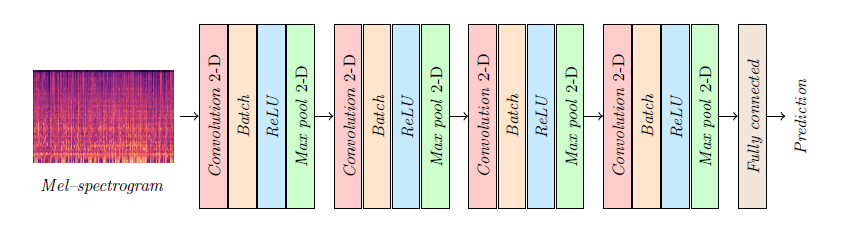
\includegraphics[scale=0.6]{images/CNN-architecture.png}
\caption{The architecture suggested by "Daniel Kostrzewa" \cite{kostrzewa2021music}.}
\label{fig:CNN-architecture}
\end{figure}

An hyper-parameter optimization has been performed on this architecture.
Not being able to do an optimization from start to finish and on all the hyper-parameters space, it has been decided to use Hyperband \cite{li2016novel} and to optimize only some hyper-parameters.

The hyper-parameters considered for the optimization were: 
\begin{itemize}
    \item The size of the kernel (fixed on each layer) in [3,6].
    \item The number of kernels for each layer in [32, 256].
    \item The probability of dropout in \{0.2, 0.25, 0.5\}.
    \item The initial learning rate in \{0.01, 0.001, 0.0001\}.
\end{itemize}

The optimization of the network has led to have, in the case without date augmentation, the first layer with 32 kernels, the second one with 128, the third with 192 and the fourth with 98. The kernel size of all layers is equal to 6. Dropout probability is 0.25 and initial learning rate is 0.001.

While in the case with data augmentation the optimization has lead to have, the first layer, the second and the third all with 64 kernels and the fourth with 96. The kernel size of all layers is equal to 4. Dropout probability is 0.25 and initial learning rate is 0.0001.

\subsection{Feature extraction with Convolutional Neural Network}

